%*******10********20********30********40********50********60********70********80

% For all chapters, use the newdefined chap{} instead of chapter{}
% This will make the text at the top-left of the page be the same as the chapter

\chap{Αξιολόγηση \& Συμπεράσματα}

Στην ενότητα αυτή, παρουσιάζονται και περιγράφονται τα πειραματικά αποτελέσματα που βρέθηκαν μέσω της αξιολόγησης του συστήματος, καθώς και οι περιορισμοί και τα συμπεράσμτα που προκύπτουν από τη χρήση του. Η δοκιμή του συστήματος αναγνώρισης της χειρονομίας "τσιμπήματος" ενσωματώθηκε στη δοκιμή ολόκληρης της εφαρμογής σκακιού και επομένως η αξιολόγηση πραγματοποιήθηκε στο σύνολο του συστήματος.


%---



\section{Αξιολόγηση}



Η παρούσα διπλωματική εργασία δίνει έμφαση στην αξιολόγηση του συστήματος που αναπτύχθηκε, δηλαδή στο σκάκι επαυξημένης πραγματικότητας.
Στη συγκεκριμένη ενότητα παρουσιάζονται τα αποτελέσμα της αξιολόησης SUS, καθώς και τα αποτελέσματα από τα ερωτηματολόγια που συμπλήρωσαν οι χρήστες μετά τις δοκιμές που πραγματοποίησαν με την εφαρμογή σκακιού επαυξημένης πραγματικότητας. Επίσης έγιναν μετρήσεις των χρόνων για την ολοκλήρωση κάθε κίνησης χειρισμού των αντικειμένων.


Συγκεκριμένα, συμμετείχαν 10 άτομα ηλικίας 20-25 ετών που γνώριζαν πώς παίζεται το επιτραπέζι παιχνίδι του σκακιού. Στην αρχή έγινε μια επεξήγηση που αφορούσε τον τρόπο λειτουργίας του συστήματος και τον τρόπο με τον οποίο πρέπει να πραγματοποιείται η χειρονομία "τσιμπήματος" για να μετακινηθεί ένα πιόνι στη σκακιέρα. Έπειτα, τους δόθηκε ένα διάστημα 1 λεπτών να εξοικειωθούν με το περιβάλλον επαυξημένης πραγματικότητας και να πραγματοποιήσουν μερικές δοκιμαστικές κινήσεις.

Οι οδηγίες που δόθηκαν στους χρήστες για την σωστή επιλογή και το χειρισμό των εικονικών αντικειμένων είχε ως εξής:
1. Τεντώστε το χέρι σας πάνω από το τραπέζι σε ύψος περίπου 15 εκατοστών.
2. Χρησιμοποιήστε το δεξί σας χέρι και πραγματοποιήστε τη χειρονομία "τσιμπήματος" κοντά σε ένα πιόνι για να το επιλέξετε. Η χειρονομία αυτή πρέπει να πραγματοποιείται με τέτοιο τρόπο, ώστε η οπή που σχηματίζεται από τον αντίχειρα και τον δείκτη να είναι πάντα ορατή από την κάμερα και τα υπόλοιπα δάκτυλα να είναι τεντωμένα και να μην πραγματοποιούν την ίδια κίνηση με τον δείκτη. Τα εικονικά πιόνι χρωματίζονται χρυσά αν επιλεγούν.
3. Μετακινήστε το πιόνι που επιλέξατε πάνω από ένα άλλο τετράγωνο της εικονικής σκακιέρας, με τον ίδιο τρόπο με τον οποίο θα παίζατε σκάκι με πραγματικά πιόνια και πραγματική σκακιέρα. 
4. Σταματήστε την χειρονομία κατά την οποία ο δείκτης και ο αντίχειρας αγγίζουν ο ένας τον άλλον, ώστε να απελευθερωθεί το αντικείμενο. Το εικονικό πιόνι θα τοποθετηθεί στο τετράγωνο που βρίσκεται πιο κοντά από το σημείο στο οποίο αφήνεται το πιόνι.


\subsection{Αξιολόγηση SUS}



Η αξιολόγηση του συστήματος αναγνώρισης χειρονομιών που αναπτύχθηκε περιορίστηκε σε ερωτήσεις προς τους χρήστες μέσω ερωτηματολογιών χρηστικότητας σε σχέση με τις χειρονομίες. Οι χρήστες δοκίμασαν για πρώτη φορά την εφαρμογή κατά το στάδιο της αξιόγησης, ωστόσο είχαν τη δυνατότητα να μάθουν πώς λειτουργεί και να εξοικειωθούν με το περιβάλλον επαυξημένης πραγματικότητας σε μία περίοδο 10 διάρκειας 10 λεπτών. Ο χρόνος αυτός θεωρήθηκε αρκετός για να μάθουν να χρησιμοποιούν το σύστημα αναγνώρισης χειρονομιών σωστά και να μπορούν να μετακινούν εικονικά πιόνια στην εικονική σκακιέρα. 


Προκειμένου να μπορέσουμε να αξιολογήσουμε τη εφαρμογή σκακιού επαυξημένης πραγματικότητας που αναπτύχθηκε, χρησιμοποιήθηκε η μέθοδος "Κλίμακας Χρησιμότητας Συστήματος" (System Usability Scale - SUS). Η μέθοδος αυτή περιλαμβάνει ένα ερωτηματολόγιο με 10 ερωτήσεις προς τους χρήστες, με στόχο τη μέτρηση της ευκολίας χρήσης ενός συστήματος λογισμικού, hardware, κινητών τηλεφώνων ή ιστοσελίδων και παρουσιάστηκε από τον John Brooke \cite{Brooke1996}.

Πρόκειται για μία τεχνολογία η οποία έχει δοκιμαστεί σε πολλές εφαρμογές και θεωρείται πλέον standard της βιομηχανίας, με αναφορές σε περισσότερες από 600 επιστημονικές δημοσιεύσεις. 


Το ερωτηματολόγιο SUS αποτελείται, όπως είπαμε, από 10 ερωτήσεις (στην αγγλική γλώσσα). Ο χρήστης καλείται να απαντήσει σε κάθε ερώτηση, κάθεμία από τις οποίες έχει 5 πιθανές απαντήσεις:


\begin{figure}[H]
    \centering
    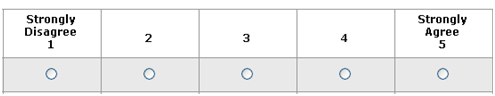
\includegraphics[width=0.9\textwidth]{Files/Figures/sus-responses.png}
    \caption[Το markerboard που δημιουργήθηκε μέσω της ArUco]{Το markerboard που δημιουργήθηκε μέσω της ArUco}
    \label{fig:markerboard}
\end{figure}




Η βαθμολογία SUS βγαίνει με τον εξής τρόπο:
\begin{description}
\item Για τις ερωτήσεις με περιττό αριθμό: Αφαιρείται μία μονάδα από την τιμή της απάντησης (1-5).
\item Για τις ερωτήσεις με άρτιο αριθμό: Αφαιρείται η τιμή της απάντησης από τον αριθμό 5.
\item  Προσθέτοντας τις τιμές των απαντήσεων για κάθε χρήστη και πολλαπλασιάζοντας το σύνολο με 2.5, παίρνουμε ένα εύρος τιμών από το 0 ως το 100.
\end{description}




Η αξιολόγηση ενός συστήματος μέσω της μεθόδου SUS θεωρείται έγκυρη και αξιόπιστη. Στόχος αυτού του συστήματος αξιολόγησης είναι να παρέχει ένα εύκολο τεστ προς συμπλήρωση στους χρήστες που δοκιμάζουν το σύστημα και να επιτρέψει συγκρίσεις μεταξύ προϊόντων και εφαρμογών, με απώτερο σκοπό την αντικειμένική αξιολόγηση της χρηστικότητας του συστήματος. 


Το αποτέλεσμα της αξιολόγησης SUS για το σύστημά μας ήταν 73.25 με τυπική απόκλιση 10.7 και μέσο 75, το οποίο με βάση το \cite{bangor2008empirical} σημαίνει ότι έχουμε ένα αποδεκτό αποτέλεσμα (χρειάζεται να έχουμε ποσοστό μεγαλύτερο από 70\%).
Τα αποτελέσματα φαίνονται στις παρακάτω εικόνες. Στην πρώτη απεικονίζονται οι απαντήσεις που έδωσε κάθε χρήστης, ενώ στη δεύτερη το συνολικό αποτέλεσμα.

\begin{center}
\begin{tabular}{ |c||p{0.6cm}|p{0.6cm}|p{0.6cm}|p{0.6cm}|p{0.6cm}|p{0.6cm}|p{0.6cm}|p{0.6cm}|p{0.6cm}|p{0.8cm}||c|  }
\hline
 \multicolumn{12}{|c|}{System Usability Scale Results} \\
\hline
User   & Q1 & Q2 & Q3 & Q4 & Q5 & Q6 & Q7 & Q8 & Q9 & Q10 & SUS Score\\
 \hline
 User1   & 4    & 2 &   4 &   1 &   4 &   2 &   5 &   4 &   4 &   2 &   75.0\\
 User2   & 3    & 2 &   3 &   2 &   3 &   3 &   3 &   3 &   2 &   2 &   55.0\\
 User3   & 3    & 2 &   4 &   1 &   4 &   3 &   5 &   1 &   4 &   1 &   80.0\\
 User4   & 5    & 1 &   4 &   1 &   4 &   1 &   5 &   1 &   4 &   1 &   92.5\\
 User5   & 3    & 1 &   4 &   1 &   4 &   2 &   4 &   2 &   4 &   1 &   80.0\\
 User6   & 4    & 2 &   4 &   3 &   4 &   2 &   3 &   3 &   4 &   2 &   67.5\\
 User7   & 2    & 1 &   3 &   1 &   5 &   2 &   4 &   2 &   3 &   1 &   75.0\\
 User8   & 2    & 2 &   2 &   1 &   4 &   2 &   4 &   3 &   2 &   2 &   60.0\\
 User9   & 2    & 2 &   3 &   1 &   4 &   1 &   4 &   2 &   3 &   2 &   70.0\\
 User10   & 3    & 1 &   3 &   1 &   5 &   2 &   4 &   2 &   3 &   1 &   77.5\\
\hline
\end{tabular}
\end{center}


\begin{figure}[H]
    \centering
    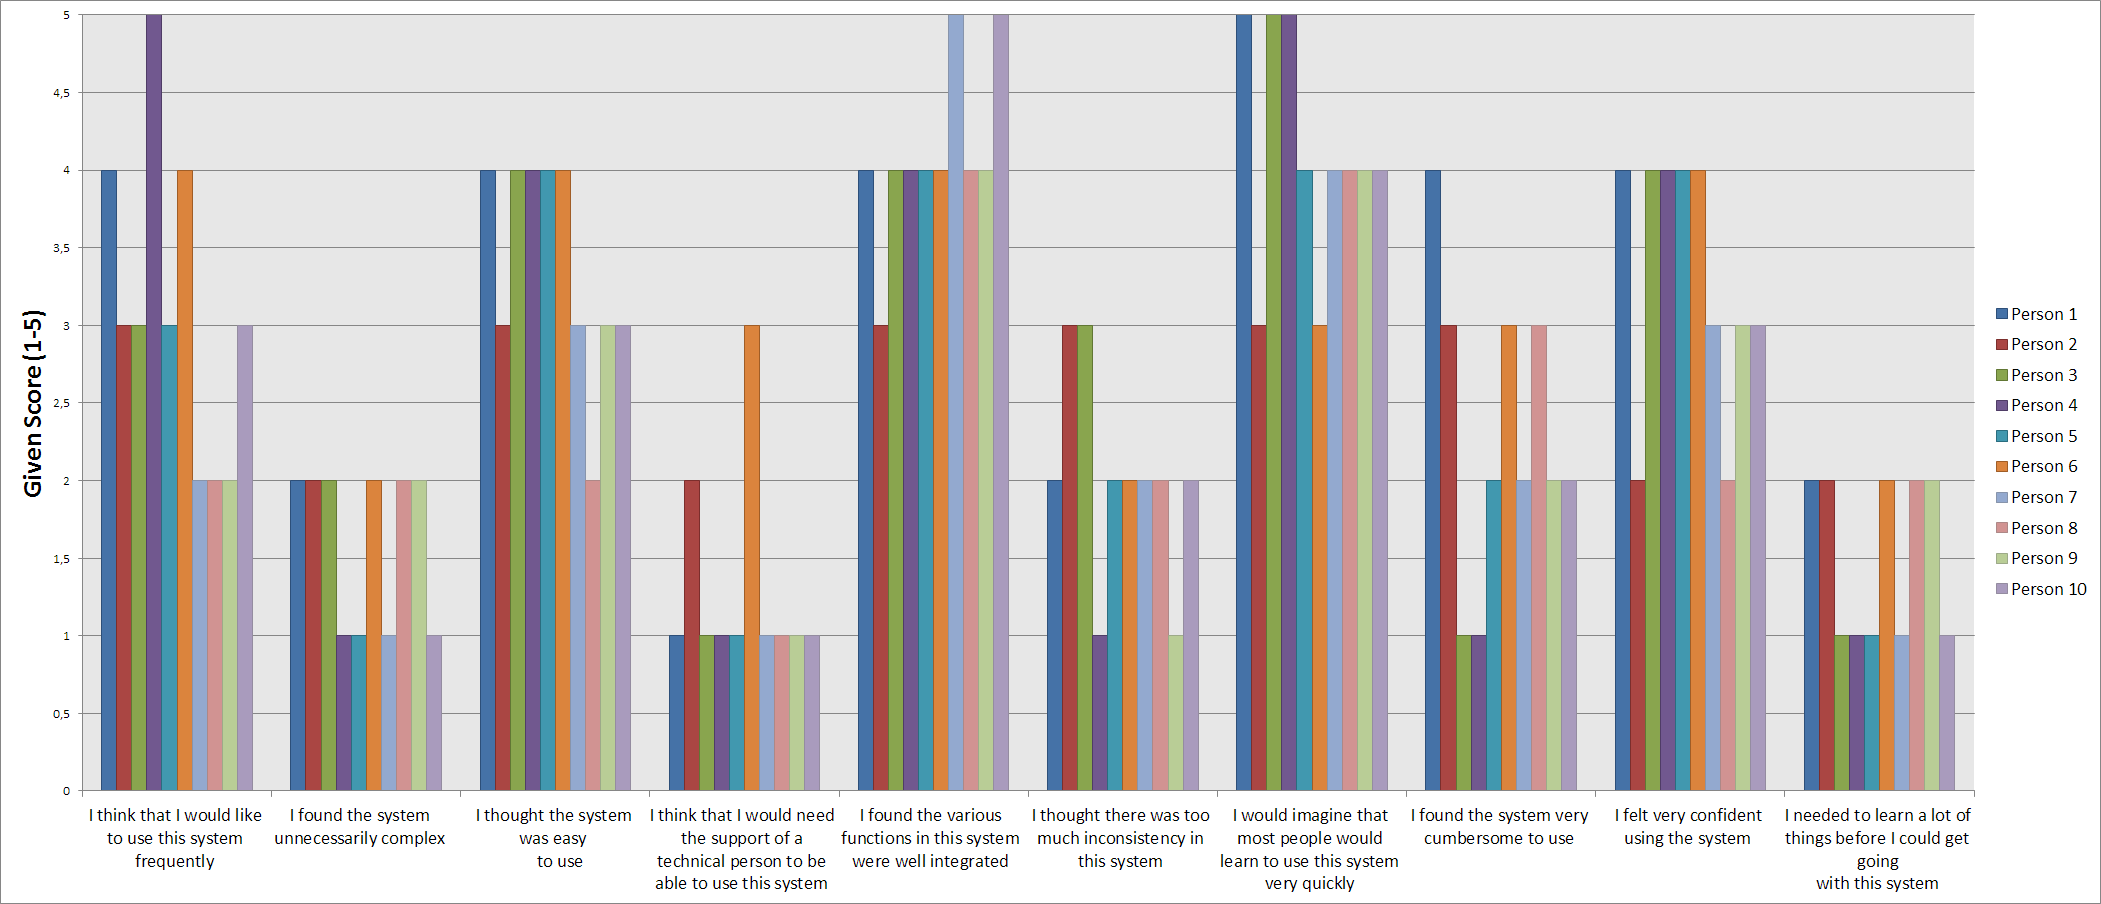
\includegraphics[width=0.95\textwidth]{Files/Figures/sus_per_person.png}
    \caption[Το markerboard που δημιουργήθηκε μέσω της ArUco]{Το markerboard που δημιουργήθηκε μέσω της ArUco}
    \label{fig:markerboard}
\end{figure}


\begin{figure}[H]
    \centering
    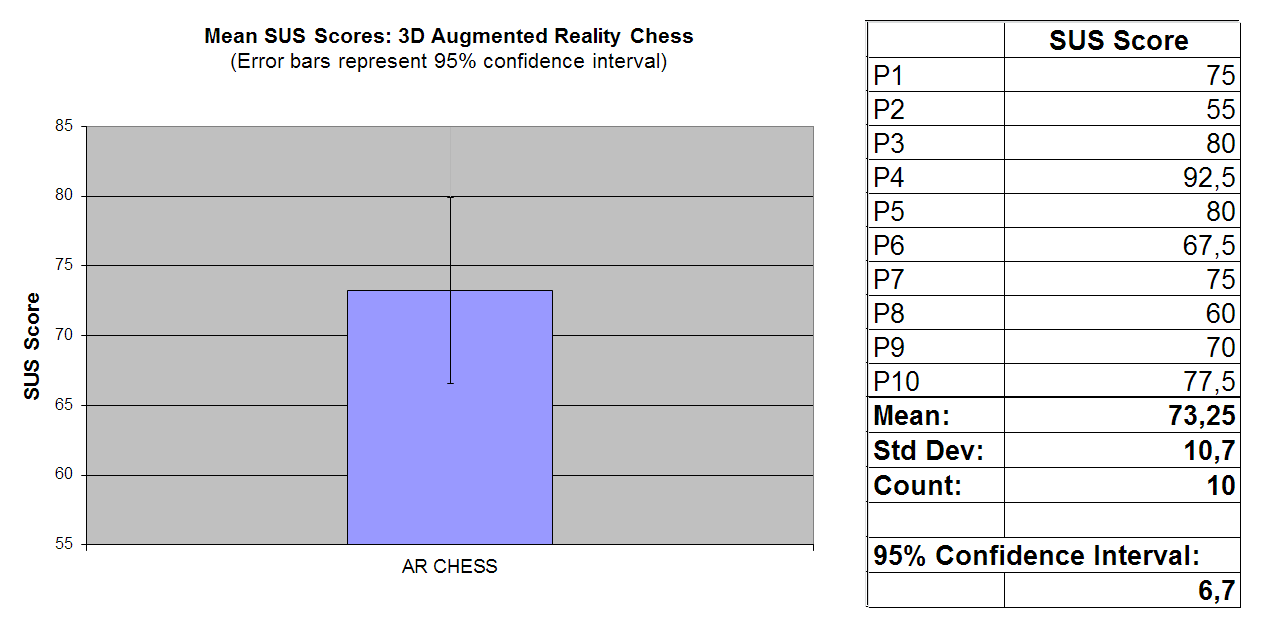
\includegraphics[width=0.95\textwidth]{Files/Figures/sus.png}
    \caption[Το markerboard που δημιουργήθηκε μέσω της ArUco]{Το markerboard που δημιουργήθηκε μέσω της ArUco}
    \label{fig:markerboard}
\end{figure}


Η αξιολόγηση έδειξε ότι το σύστημα είναι χρηστικό ως μηχανισμός εισόδου σε μία διεπαφή επαυξημένης πραγματικότητας στον τρισδιάστατο χώρο, παρά το γεγονός ότι το σύστημα δεν έχει βελτιστοποιηθεί ακόμα ως προς τη λειτουργικότητά του, αφού οι χρήστες μπόρεσαν επιτυχημένα να μετακινήσουν τα πιόνια στη σκακιέρα και να παίξουν ενάντια στον υπολογιστή. 




\subsection{Χρόνος και Επιτυχία Ολοκλήρωσης Κινήσεων}


Στην πρώτη φάση της αξιολόγησης, μετρήσαμε τον αριθμό των χειρονομιών "τσιμπήματος" που χρειάστηκε να κάνει κάθε χρήστης μέχρι να γίνει η σωστή επιλογή του εικονικού αντικειμένου. Πέρα από αυτό, έγινε μέτρηση του χρόνου που χρειάστηκε κάθε χρήστης για να μετακινήσει ένα εικονικό πιόνι από τη στιγμή που το επέλεξε. Τέλος, θέλαμε να βρούμε κατά πόσο το σύστημα μας είναι αξιόπιστο, δηλαδή κατά πόσο το σύστημά μας καταλαβαίνει, με βάση την κίνηση του χρήστη, σε ποιο τετράγωνο θέλησε ο χρήστης να αφήσει το πιόνι, όπως αναφέρθηκε και σε προηγούμενη ενότητα. Τα αποτελέσματα φαίνονται στον παρακάτω πίνακα.


\begin{table}[h]
\centering
\caption{My caption}
\label{my-label}
\begin{tabular}{|r|r|r|r|r|r|r|}
\hline
\multicolumn{1}{|c|}{{\bf \begin{tabular}[c]{@{}c@{}}Participant\\   \#\end{tabular}}} & \multicolumn{1}{c|}{{\bf \begin{tabular}[c]{@{}c@{}}Time per \\ Correct Move\\   (sec)\end{tabular}}} & \multicolumn{1}{c|}{{\bf \begin{tabular}[c]{@{}c@{}}Tasks Completed\\   (out of 30)\end{tabular}}} & \multicolumn{1}{c|}{{\bf Time \%}} & \multicolumn{1}{c|}{{\bf Tasks \%}} & \multicolumn{1}{c|}{{\bf SUS Rating \%}} & \multicolumn{1}{c|}{{\bf Average}} \\ \hline
1                                                                                      & 2,99                                                                                                  & 25                                                                                                 & 83\%                               & 83\%                                & 75\%                                     & 81\%                               \\ \hline
2                                                                                      & 4,23                                                                                                  & 25                                                                                                 & 59\%                               & 83\%                                & 55\%                                     & 66\%                               \\ \hline
3                                                                                      & 3,05                                                                                                  & 16                                                                                                 & 82\%                               & 53\%                                & 80\%                                     & 72\%                               \\ \hline
4                                                                                      & 4,94                                                                                                  & 25                                                                                                 & 50\%                               & 83\%                                & 92,5\%                                   & 75\%                               \\ \hline
5                                                                                      & 3,49                                                                                                  & 25                                                                                                 & 71\%                               & 83\%                                & 80\%                                     & 78\%                               \\ \hline
6                                                                                      & 5,64                                                                                                  & 22                                                                                                 & 44\%                               & 73\%                                & 67,5\%                                   & 62\%                               \\ \hline
7                                                                                      & 2,49                                                                                                  & 18                                                                                                 & 100\%                              & 60\%                                & 75\%                                     & 78\%                               \\ \hline
8                                                                                      & 4,66                                                                                                  & 28                                                                                                 & 53\%                               & 93\%                                & 60\%                                     & 69\%                               \\ \hline
9                                                                                      & 2,74                                                                                                  & 28                                                                                                 & 91\%                               & 93\%                                & 70\%                                     & 85\%                               \\ \hline
10                                                                                     & 3,00                                                                                                  & 26                                                                                                 & 83\%                               & 87\%                                & 77,5\%                                   & 82\%                               \\ \hline
{\bf Averages}                                                                         & {\bf 3,723}                                                                                           & {\bf 23,8}                                                                                         & {\bf 72\%}                         & {\bf 79\%}                          & {\bf 73\%}                               & {\bf 75\%}                         \\ \hline
\end{tabular}
\end{table}





\begin{figure}[H]
    \centering
    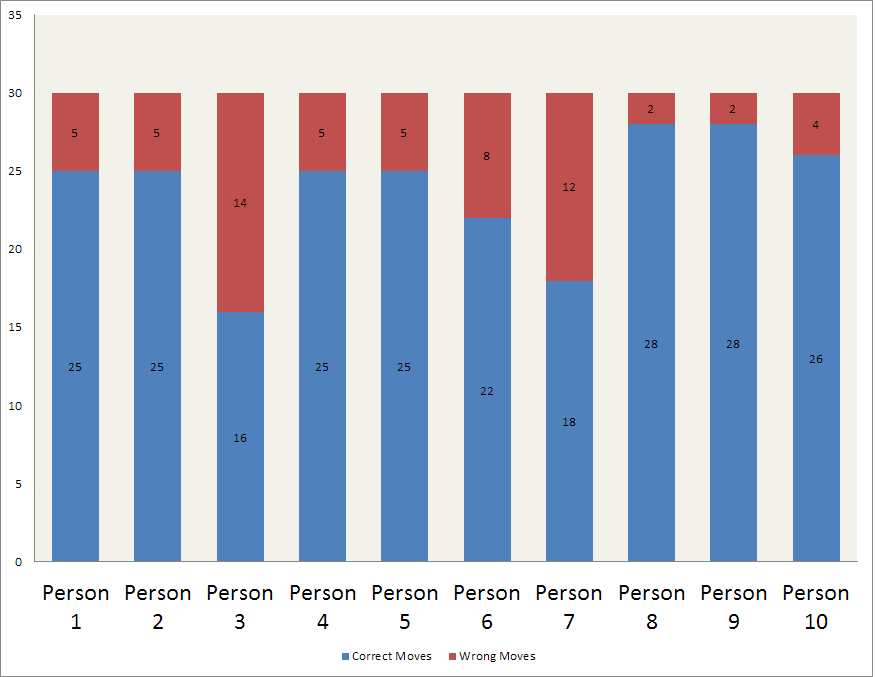
\includegraphics[width=0.95\textwidth]{Files/Figures/correctmoves.png}
    \caption[Το markerboard που δημιουργήθηκε μέσω της ArUco]{Το markerboard που δημιουργήθηκε μέσω της ArUco}
    \label{fig:markerboard}
\end{figure}



Παρά το γεγονός ότι οι διαδοχικές κινήσεις ενός παίκτη στο σκάκι, συνήθως δεν έχουν κάποια συνοχή, τα αποτελέσματα κρίνονται ιδιαίτερα ικανοποιητικά. Ο μέσος χρόνος εκτέλεσης μιας κίνησης βρέθηκε κοντά στα 3.7 δευτερόλεπτα, επομένως μπορούμε να πούμε ότι η αλληλεπίδραση του χρήστη με το σύστημα φαίνεται αρκετά φυσική. Ωστόσο, παρατηρήθηκε ότι οι λανθασμένες κινήσεις ξεπέρασαν τις προσδοκίες μας, ειδικά όταν οι χρήστες προσπαθούσαν να πραγματοποιήσουν μεγάλες κινήσεις σε αποστάσεις μεγαλύτερες των 3 τετραγώνων της σκακιέρας. Για το συγκεκριμένο λόγο, προτάθηκε μία λύση, η οποία παρουσιάζεται στην ενότητα~\ref{sec:conclusion}


\subsection{Ερωτηματολόγια}

Για να μπορέσουμε να αξιολογήσουμε με περισσότερη ακρίβεια το σύστημα που αναπτύχθηκε και την εμπειρία των χρηστών, μοιράστηκε στους χρήστες που δοκίμασαν την εφαρμογή ένα ανοιχτό ερωτηματολόγιο, το οποίο συμπλήρωσαν αμέσως μετά την αξιολόγηση SUS και το τέλος της δοκιμής. Ζητήθηκε από τους χρήστες να δηλώσουν παρόμοιες εμπειρίες με εφαρμογές επαυξημένης πραγματικότητας και συστήματα αλληλεπίδρασης μέσω χειρονομιών. Το ερωτηματολόγιο που μοιράστηκε, αφορούσε την εμπειρία των χρηστών ως προς την απόδοση της αναγνώρισης χειρονομιών του συστήματος και το επίπεδο "εμβύθισής" τους στο περιβάλλον επαυξημένης πραγματικότητας. 


Οι περισσότεροι χρήστες από αυτούς που δοκίμασαν την εφαρμογή δεν είχαν παρόμοια εμπειρία ούτε από χρήση συστημάτων επαυξημένης πραγματικότητας, ούτε από συστήματα αναγνώρισης χειρονομιών.
Όσον αφορά την απόκριση της συστήματος ως προς την αναγνώριση των χειρονομιών, οι περισσότεροι χρήστες θεώρησαν ότι πραγματοποιείται αρκετά άμεσα, ενώ παράλληλα θεώρησαν ότι η απεικόνιση των αντικειμένων με βάση το χάρτη βάθους της σκηνής εξυπηρετεί το σκοπό της εφαρμογής που είναι η "εμβύθιση" του χρήστη και η ευκολία επιλογής των πιονιών, προσφέροντας μία ρεαλιστική εμπειρία.

Συγκεκριμένα ως προς το χειρισμό των εικονικών αντικειμένων, οι χρήστες απάντησαν θετικά ως προς την ευκολία επιλογής ενός εικονικού πιονιού στο περιβάλλον της εφαρμογής, αλλά και ως προς την ευκολία μετακίνησής του στη σκακιέρα. Η πειραματική εγκατάσταση που χρησιμοποιήθηκε με το καπέλο και το markerboard μπροστά από το χρήστη φαίνεται ότι δεν δυσκόλεψε το χρήστη, αφού δεν περιλαμβάνονταν περιττά καλώδια ή περισσότερα markers, παρά μόνο τα χέρια τους για τη μετακίνηση των εικονικών αντικειμένων.


Τα ερωτηματολόγια έδειξαν ότι η χρήση της εφαρμογής δεν κούρασε τους χρήστες, ούτε το γεγονός ότι έπρεπε να πραγματοποιούν τη χειρονομία "τσιμπήματος" τοποθετώντας το χέρι τους με τέτοιο τρόπο ώστε η οπή που σχηματίζεται ανάμεσα σε δείκτη και αντίχειρα να βρίσκεται κάθεται προς τον αισθητήρα. Ουσιαστικά αρκούσε η ανάδραση που έπαιρναν από το σύστημα που δεν τους επέτρεπε να επιλέξουν ένα πιόνι, αν δεν πραγματοποιούσαν σωστά τη χειρονομία "τσιμπήματος". 

\begin{figure}[H]
    \centering
    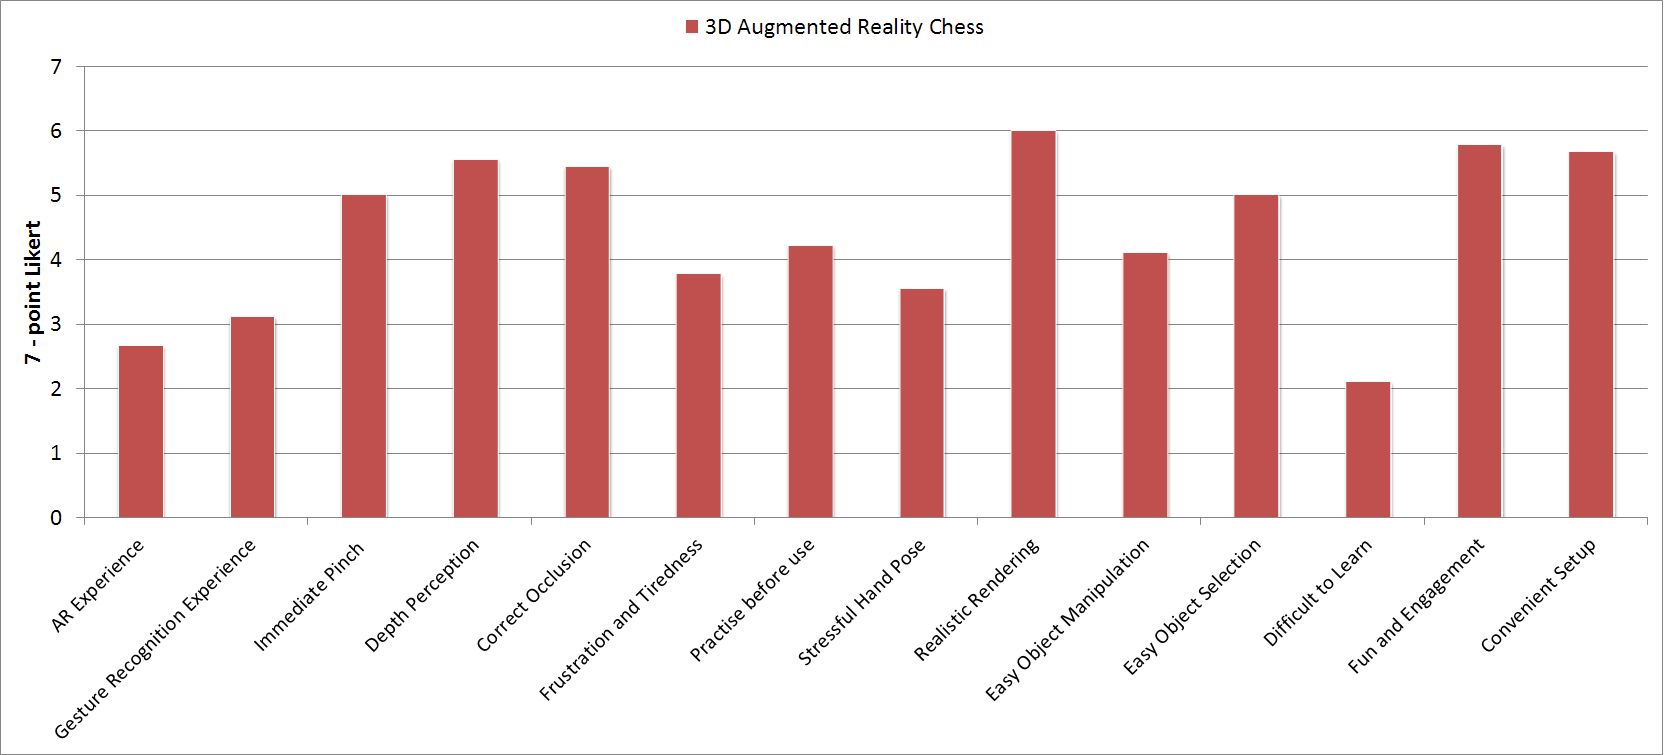
\includegraphics[width=0.9\textwidth]{Files/Figures/questionnaire.png}
    \caption[Το markerboard που δημιουργήθηκε μέσω της ArUco]{Το markerboard που δημιουργήθηκε μέσω της ArUco}
    \label{fig:markerboard}
\end{figure}




Οι χρήστες που δοκίμασαν να επιλέξουν σιγά σιγά τα πιόνια και μετά να δοκιμάσουν να τα μετακινήσουν, δεν είχαν κάποιο πρόβλημα και βελτιώθηκαν στη χρήση του συστήματος με το χρόνο, ενώ όσοι προσπάθησαν βιαστικά να τα επιλέξουν κουράστηκαν κατά τη διάρκεια του παιχνιδιού. Η πλειονότητα, πάντως, των ατόμων που δοκίμασαν την εφαρμογή συμφώνησε πως είναι απαραίτητη η εξάσκηση για τη χρήση του συστήματος σε ένα αρχικό στάδιο. Από εκεί και πέρα, ωστόσο, η διαδικασία απλοποιείται. Εξάλλου, κάθε νέα συσκευή ή τρόπος αλληλεπίδρασης με ένα σύστημα απαιτεί ένα χρονικό διάστημα για τη μάθηση της χρήσης του.


Την υψηλότερη βαθμολογία, στο ερωτηματολόγιο που δόθηκε στους χρήστες, συγκέντρωσε η ερώτηση σχετικά με το αν η εφαρμογή σκακιού που αναπτύχθηκε τους φάνηκε διασκεδαστική. Η υψηλή αυτή βαθμολογία δείχνει ότι η εφαρμογή που παρουσιάζεται στη συγκεκριμένη διπλωματική εργασία πετυχαίνει το στόχο της σχετικά με τη φυσική αλληλεπίδραση με το χρήστη και τη μεταφορά ενός κλασικού επιτραπέζιου παιχνιδιού σε περιβάλλον επαυξημένης πραγματικότητας.


Ίσως το κυριότερο πρόβλημα της εφαρμογής, λόγω της πειραματικής εγκατάστασης που χρησιμοποιήθηκε, βρίσκεται στην αίσθηση του βάθους στην επαυξημένη σκηνή, ως προς το σημείο παρατήρησης του χρήστη. Αυτό σημαίνει ότι, ενώ ο χρήστης είναι σίγουρος ότι το εικονικό αντικείμενο κινείται μέσω του χεριού του προς τα πίσω, στην πραγματικότητα κινείται προς τα πάνω. Όπως είπε ακριβώς ένας από τους χρήστες :"Όταν κατανοήσω που ακριβώς βρίσκεται το πιόνι στο χώρο κοιτώντας το markerboard, μπορώ να καταλάβω προς τα πού πρέπει να κινήσω το χέρι μου, το οποίο κρατάει το πιόνι στον εικονικό κόσμο.". Αυτή η σκέψη ήταν κοινή για αρκετούς από τους συμμετέχοντες και θεώρησαν ότι η χρήση ενός συστήματος Video See-Through HMD θα ήταν ιδανική για το σύστημα, αφού θα κοίταζαν προς το markerboard και θα έβλεπαν τα εικονικά πιόνια μέσω του HMD, επομένως θα μπορούσαν να έχουν καλύτερη αίσθηση του βάθους, σε σχέση με τη χρήση μιας οθόνης για την επαύξηση της σκηνής.



Τέλος, κάποιοι από τους χρήστες που δοκίμασαν την εφαρμογή και πρότειναν βελτιώσεις, θεώρησαν ότι μπορεί να βελτιωθεί το επίπεδο της απόκρυψης των αντικειμένων (occlusion) αν εφαρμοστεί κάποιο φίλτρο εξομάλυνσης στο χάρτη βάθους του αισθητήρα.







\section{Συμπεράσματα και Παρατηρήσεις} \label{sec:conclusion}


Κατά τη διάρκεια των δοκιμών προσομοίωσης του σκακιού της επαυξημένης πραγματικότητας που αναπτύχθηκε, παρουσιάστηκαν ορισμένοι περιορισμοί και μειονεκτήματα του συστήματος αλληλεπίδρασης, τα οποία οδήγησαν στον επανασχεδιασμό ορισμένων πτυχών της εφαρμογής. 


Αρχικά, αν κατά τη διαδικασία εξαγωγής blobs για την ανίχνευση του χεριού του χρήστη, αυτός αποφασίσει να επιλέξει ένα αντικείμενο και να το μετακινήσει, το χέρι του μπορεί να βρίσκεται πολύ κοντά στο τραπέζι. Αυτό έχει σαν αποτέλεσμα την αποτυχία αναγνώρισης της χειρονομίας "τσιμπήματος", αφού το πρόγραμμα θεωρεί το χέρι και τα δάκτυλα του χρήστη μαζί με το τραπέζι ή την επιφάνεια όπου βρίσκεται το markerboard ως ένα blob, συνολικά. Το ίδιο συμβαίνει αν χέρι του χρήστη είναι ορατό από τον αισθητήρα αλλά το μπράτσο του είναι κοντά στο τραπέζι με αποτέλεσμα μπράτσο, χέρι και τραπέζι να θεωρούνται ως ένα blob. Τότε το σύστημα, το οποίο προσπαθεί να βρει το κοντινότερο blob, μπορεί να μπερδευτεί και να μην μπορέσει να ανιχνεύσει κάποια Το πρόβλημα αυτό εμφανίζεται και σε άλλους αισθητήρες που χρησιμοποιούν παρόμοιες προσεγγίσεις αναγνώρισης χειρονομιών, όπως το Leap Motion. Ωστόσο, θεωρήθηκε ότι θα ήταν υπερβολικό να αλλάξουμε εντελώς τον τρόπο με τον οποίο το RealSense SDK εξάγει τα blobs. Αντίθετα, σκεφτήκαμε ότι μπορούμε να αντιμετωπίσουμε το πρόβλημα με τον οπτικό σχεδιασμό μιας εικονικής σκακιέρας που είναι συνήθως ένα κυβικό σχήμα, δηλαδή έχει ένα ορισμένο ύψος πάνω από την επιφάνεια του τραπεζιού. Συνεπώς, στην εφαρμογή του σκακιού επαυξημένης πραγματικότητας που παρουσιάζεται, απεικονίζεται μία σκακιέρα κάτω από τα εικονικά πιόνια, η οποία αποτελείται από μία διάταξη πολλαπλών κύβων με ύψος περίπου 3,5cm, αφού αυτό είναι το όριο ύψους πάνω από το οποίο μπορεί ο αισθητήρας να ανιχνεύσει σωστά το χέρι του χρήστη. 


Ακόμα ένα πρόβλημα που παρουσιάστηκε κατά τη διάρκεια των δοκιμών, αφορά το γεγονός ότι η λανθασμένη ανίχνευση του σημείου στο οποίο συνέβη η χειρονομία "τσιμπήματος" μπορεί να οδηγήσει στην ακούσια κίνηση ενός εικονικού πιονιού σε διαφορετική θέση από αυτή που επιδιώκει ο χρήστης. Τα αποτελέσματα έδειξαν ότι οι χρήστες συχνά εξέφραζαν παράπονα για το συγκεκριμένο πρόβλημα Για παράδειγμα, ο χρήστης μπορεί να ήθελε να μετακινήσει ένα απλό πιόνι - στρατιώτη 2 τετράγωνα μακριά από την αρχική του θέση. Ωστόσο, κατά τη διάρκεια αυτής της μετατόπισης, μπορεί σε κάποιο frame να μην ανιχνευόταν η χειρονομία "τσιμπήματος" και το σύστημα θεωρούσε ότι ο χρήστης ήθελε να απελευθερώσει το πιόνι νωρίτερα. Έτσι το σύστημα αποκρινόταν, αφήνοντας το πιόνι στο προηγούμενο τετράγωνο από αυτό το οποίο επιθυμούσε ο χρήστης. Το γεγονός, μάλιστα, ότι το πρόγραμμά μας στη συνέχεια, μπαίνει σε κατάσταση γύρου του αντιπάλου, δηλαδή του υπολογιστή, δεν αφήνει περιθώρια στο χρήστη να διορθώσει το λάθος του. 


Θεωρήσαμε, λοιπόν, ότι είναι καλύτερο να υλοποιηθεί ένας αλγόριθμος, ο οποίος θα ελέγχει αν ο χρήστης πραγματοποίησε απελευθέρωση ενός πιονιού (pinch-out) με περισσότερη ακρίβεια. Για να συμβεί αυτό, δημιουργήσαμε έναν buffer ο οποίος καταγράφει έναν αριθμό διαδοχικών frames που ορίζεται ως παράμετρος στο πρόγραμμα. Αν κάθε στοιχείο του buffer έχει καταγράψει κατάσταση απελευθέρωσης πιονιού, τότε θεωρείται ότι έχει όντως πραγματοποιηθεί απελευθέρωση πιονιού από το χρήστη και επομένως η εφαρμογή μας πρέπει να μετακινήσει το πιόνι στο νέο τετράγωνο αν η κίνηση είναι έγκυρη. Σε διαφορετική περίπτωση, αν έστω και ένα στοιχείο του buffer δε βρίσκεται σε κατάσταση "pinch-out", τότε το σύστημα παραμένει σε κατάσταση "pinch-continuous". Στην ενότητα \ref{s:rendering}, παρουσιάζεται το σύστημα με τον buffer που αναφέραμε. 



Ορισμένοι περιορισμοί της προσέγγισης σχεδιασμού της εφαρμογής που παρουσιάστηκε αφορούν τη θέση και τον προσανατολισμό των χεριών του χρήστη. Όταν ο χρήστης προσπαθήσει να επιλέξει, δηλαδή να "τσιμπήσει" ένα πιόνι με τη χειρονομία που παρουσιάστηκε στην ενότητα \ref{section:pinch}, μπορεί να αποτύχει, αν ο προσανατολισμος του χεριού δεν είναι ο επιθυμητός. Αυτό συμβαίνει όταν ο χρήστης τοποθετεί το χέρι του κάθετα προς τον αισθητήρα, αφού η οπή που δημιουργείται από τον αντίχειρα και το δείκτη, δεν είναι εμφανής στο πεδίο όρασης του αισθητήρα.




Παρά το γεγονός, ότι για να λειτουργήσει σωστά η εφαρμογή σκακιού που αναπτύχθηκε και για να αυξηθεί το επίπεδο "εμβύθισης" του χρήστη, είναι η χρήση ενός συστήματος video see-through HMD. Όπως αναφέρθηκε και σε προηγούμενες ενότητες, θα μπορούσαμε να τοποθετήσουμε τον αισθητήρα πάνω στο Oculus Rift και να απεικονίσουμε την επαυξημένη σκηνή στην μικρή οθόνη που βρίσκεται μέσα του. Ωστόσο, λόγω χρονικών περιορισμών, η δημιουργία ενός τέτοιου συστήματος δεν κατέστη δυνατή. Για το λόγο αυτό, αποφασίστηκε η υλοποίηση ενός συστήματος, όπου ο χρήστης θα βλέπει την επαυξημένη σκηνή στην οθόνη ενός υπολογιστή για να αποδειχτεί η ορθότητα του συστήματος. 






 The new results showed that our algorithm performed well along the attempts although there were random results in the attempts that does not reflect precisely if it was easier or not, - in general, this behaviour was seen in both cases- concluding that actually there is a decrease on time of each attempt when performing the gesture, validating the learnability aspect in the gesture performance, but not when moving the object to the specified area, in this case, the results were very smooth, meaning that the average time it took to grab-move-release was almost the same in all the samples. Furthermore, when comparing these results within both algorithms we found that there was a relevant improvement with our algorithm, validating our first assumption made, but on different events in the scene. On the qualitative results, the agreement with the learning effect statement is mutual among the users that stated to improve at some level on each attempt while on the SUS, the detection of problems that influenced our results corroborates the dispersion of data we have, specially during the grabbing task -that can be inferred from the time it took- that it was more difficult to initiate the grabbing action than manipulating the object with it. One problem that affected the performance initially was the depth perception of the users, where the point of view of the camera did not help the user to perceive the exact location of the objects in the z-axis(depth) and y-axis(height), even when the farther objects were smaller than the closer ones, it was observed that users struggle with this problem frequently; just after recognizing the environment, users take the tabletop marker as a reference to infer the locations above it, this achievement is important, as it shows the inner relationship between the real and virtual worlds perceived by the users, however, the awareness was not immediate and in this sense, more visual cues should guide the user through the augmentation to offer the perception of depth in a proper way like illumination and shadowing[55] or meshes on the scene[32]. 